%! Concluding a Test for a Population Proportion — Unit 6, Lesson 6.6 — Guided Notes (Answer Key)
\documentclass[10pt]{article}
\usepackage{apstats-article}
\usepackage{apstats-key}   % pulls in -boxes; do NOT also load -boxes
\newcommand{\TallMath}[1]{$\displaystyle #1\rule[-1.4em]{0pt}{3.2em}$}

\begin{document}

\pageheader{Unit 6, Lesson 6.6}{Guided Notes --- Answer Key}
\namedateperiod

\vspace{0.15in}

\begin{objectivebox}
Make and justify a formal reject/fail-to-reject decision and write a complete conclusion in
context using the four-step procedure.
\end{objectivebox}

\begin{vocabbox}
\begin{description}
  \item[\termblanklong{Significance level} $\alpha$] The pre-chosen probability threshold; reject
        $H_0$ when $p\text{-value} \le$ \ans{$\alpha$}. Common: $\alpha =$ \ans{0.05} (default).
  \item[\termblanklong{Reject $H_0$}] Decision when $p\text{-value}$ \ans{$\le$} $\alpha$; data provide
        sufficient evidence \ans{for $H_a$}.
  \item[\termblanklong{Fail to reject $H_0$}] Decision when $p\text{-value}$ \ans{$>$} $\alpha$; insufficient
        evidence \ans{against $H_0$}. \textbf{Never say ``accept $H_0$.''}
  \item[\termblanklong{Statistically significant}] A result is significant at level $\alpha$ if
        $p\text{-value} \le$ \ans{$\alpha$}.
\end{description}
\end{vocabbox}

\begin{notesbox}{Decision Rule}
\begin{center}
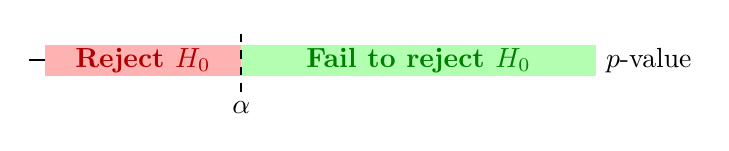
\begin{tikzpicture}
  \draw[thick,->] (-0.2,0) -- (7,0) node[right] {$p$-value};
  \fill[red!30] (0,-0.2) rectangle (2.5,0.2);
  \fill[green!30] (2.5,-0.2) rectangle (7,0.2);
  \draw[dashed,thick] (2.5,-0.4) -- (2.5,0.4);
  \node at (2.5,-0.6) {$\alpha$};
  \node[red!70!black] at (1.25,0) {\textbf{Reject $H_0$}};
  \node[green!50!black] at (4.75,0) {\textbf{Fail to reject $H_0$}};
\end{tikzpicture}
\end{center}
\end{notesbox}

\begin{notesbox}{Conclusion Template}
\textbf{Part 1 (Decision):} ``Because $p$-value $=$ \ans{[value]} [$ \le$ / $>$] $\alpha = $ \ans{[value]},
we [reject / fail to reject] $H_0$.''\\[6pt]
\textbf{Part 2 (Context):} ``We [have / do not have] sufficient evidence that \ans{[restate $H_a$ in plain language]}.''\\[6pt]
\textbf{Avoid:} \textbf{$\times$} ``Accept $H_0$'' \quad \textbf{$\times$} ``Prove $H_a$'' \quad \textbf{$\times$} Omitting context
\end{notesbox}

\begin{notesbox}{Worked Example: Driving Test}
$p\text{-value}\approx0.145$; $\alpha=0.05$.

\textbf{Conclude:} Because $p$-value $=$ \ans{0.145} \ans{$>$} $\alpha = 0.05$, we
\ans{fail to reject} $H_0$. We \ans{do not have} sufficient evidence that the true proportion of 16-year-olds
who pass the driving test on the first attempt is \ans{less than} 50\%.
\end{notesbox}

\begin{practicebox}
Factory: $p\text{-value}=0.031$; $\alpha=0.05$.

\textbf{Conclude:} Because $p$-value $=$ \ans{0.031} \ans{$\le$} $\alpha = 0.05$, we
\ans{reject} $H_0$. We \ans{have} sufficient evidence that the true defect rate is
\ans{greater than} 15\%.
\end{practicebox}

\end{document}
